\begin{frame}
  \begin{center}
    \large{1. Évaluation d'un modèle}
  \end{center}
\end{frame}


\begin{frame}
  \frametitle{1.1 Généralisation et surapprentissage}
  \begin{itemize}
  \item[] \blue{Défi principal} de l'apprentissage supervisé :
    \begin{itemize}
    \item Il est relativement facile d'entraîner un modèle qui « marche » bien
      (faible erreur de prédiction) sur les données d'apprentissage
    \item[] Exemple extrême : apprentissage « par c\oe{}ur »
      \vspace{.5em}
    \pause
    \item \red{Généralisation :} capacité du modèle à \blue{faire de
        bonnes prédictions sur des données dont on ne connaît pas l'étiquette} 
      \vspace{.5em}
    \pause
    \item \red{Surapprentissage :} quand la performance est meilleure sur
      les données d'apprentissage que sur de nouvelles données \textcolor{gray!70}{(overfitting)}
    \end{itemize}
  \end{itemize}
\end{frame}

\begin{frame}
  \frametitle{Surapprentissage}
  Simulation : vrai modèle = polynôme de degré 3 + bruit.
  \begin{center}
    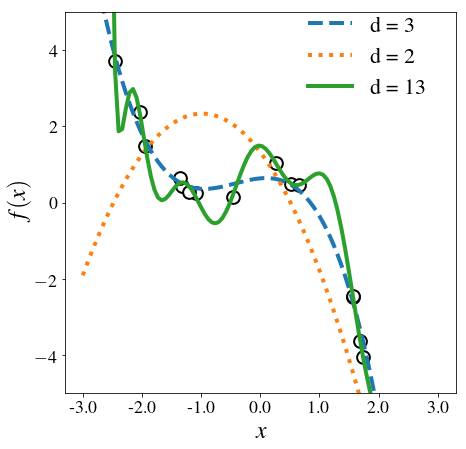
\includegraphics[width=.7\textwidth]{figures/overfit_regr}
  \end{center}
\end{frame}

\begin{frame}
  \frametitle{Compromis biais-variance}
  \begin{itemize}
    \item On considère l'erreur $\rcal(f)$ d'un modèle prédictif $f$, et les termes d'erreur suivantes : 
    \begin{itemize}
    \item \red{Erreur incompressible} : $\rcal^{\ast}$ est l'erreur qui serait faite par n'importe quel modèle.
    \item \red{Erreur d'approximation} : $\min_{h \in \fcal}\rcal(h) - \rcal^{\ast}$ 
    \item \red{Erreur d'estimation} : $\rcal(f) - \min_{h \in \fcal}\rcal(h)$
  \end{itemize}
    \item On peut écrire alors : 
    \item[] $\rcal(f) - \rcal^{\ast} = (\rcal(f) - \min_{h \in \fcal}\rcal(h)) + (\min_{h \in \fcal}\rcal(h) - \rcal^{\ast})$
    \item L'erreur totale est donc due au manque de capacité d'approcher l'erreur incompressible, car l'espace des hypothèses est trop restraint, et par la difficulté de trouver le meilleur modèle dans l'espace des hypothèses. 
    \item Il faut donc trouver un compromis entre le biais (erreur d'approximation) et la variance (erreur d'estimation). 
  \end{itemize}
\end{frame}

\begin{frame}
  \frametitle{1.2 Jeux d'entraînement et de test}
  \begin{itemize}
  \item\red{Erreur de généralisation :} erreur que l'on peut attendre sur de nouvelles
    données (la définition formelle fait appel à l'espérance)
  \pause
  \item Elle est \blue{estimée} en 
    \blue{mettant de côté} une partie des données :
    \begin{itemize}
    \item On sépare les données en un \red{jeu d'entraînement} et un \red{jeu de test} (typiquement, 80\%--20\%)
    \pause
    \begin{center}
      \begin{tikzpicture}
        \draw [draw=MyBlue, thick] (0.,5.5) rectangle (10.,4.5) node[pos=.5]{\blue{Jeu de données}};
        \draw [->, draw=MyDarkGrey, line width=1.5] (5, 4.3) -- (5, 3.8);
        \draw [draw=MyDarkGrey, thick] (0.,3.5) rectangle (8.,2.5) node[pos=.5]{\black{Entraînement}};
        \draw [draw=MyDarkGrey, thick] (8.,3.5) rectangle (10.,2.5)  node[pos=.5]{\black{Test}};
      \end{tikzpicture}
    \end{center}
    \item Le \red{jeu d'entraînement} \textcolor{gray!70}{(train set)} sert à apprendre le modèle
    \item Le \red{jeu de test} sert à estimer l'erreur de généralisation du modèle
    \end{itemize}
  \end{itemize}
\end{frame}

\begin{frame}
  \frametitle{Règle d'or}
  \begin{center}
    \red{NE PAS TOUCHER au jeu de test} \\ sauf pour évaluer l'erreur de généralisation du modèle
  \end{center}
\end{frame}

\begin{frame}
  \frametitle{1.3 Validation croisée}
  \begin{itemize}
  \item La \red{validation croisée} \textcolor{gray!70}{(cross-validation)} permet :
    \begin{itemize}
    \item d'utiliser toutes les données pour l'entraînement et pour la validation
    \item d'obtenir une performance moyenne (+/- écart-type)  moins sensible au choix du jeu de test
    \end{itemize}
  \item On sépare le jeu de données en K \blue{blocs} \textcolor{gray!70}{(folds)}
    \begin{itemize}
    \item[] En pratique, K=5 ou K=10 le plus souvent (équilibre entre le nombre
      d'expériences et la taille de chaque jeu d'entraînement)
    \end{itemize}
  \item On utilise tour à tour chacun des blocs comme \blue{jeu de
      validation} et l'union des autres comme \blue{jeu d'entraînement}
  \item[$\Rightarrow$] K scores de performance $\rightarrow$ \blue{performance de généralisation} du modèle
  \end{itemize}
\end{frame}

\begin{frame}
  \frametitle{1.3 Validation croisée}
  \begin{center}
    \small
    \begin{tikzpicture}
      \draw [draw=MyBlue, thick] (0, 6.5) rectangle (7.5, 6) node[pos=.5]{\blue{Jeu de données}};
      \pause
      \draw [->, draw=MyDarkGrey, line width=1.5] (3.75, 5.9) -- (3.75, 5.4);
      \draw [draw=MyDarkGrey, thick] (0.,5.3) rectangle (1.5,4.8) node[pos=.5]{\black{Bloc 1}};
      \draw [draw=MyDarkGrey, thick] (1.5,5.3) rectangle (3.,4.8) node[pos=.5]{\black{Bloc 2}};
      \draw [draw=MyDarkGrey, thick] (3.,5.3) rectangle (4.5,4.8) node[pos=.5]{\black{Bloc 3}};
      \draw [draw=MyDarkGrey, thick] (4.5,5.3) rectangle (6.,4.8) node[pos=.5]{\black{Bloc 4}};
      \draw [draw=MyDarkGrey, thick] (6.,5.3) rectangle (7.5,4.8) node[pos=.5]{\black{Bloc 5}};
      \pause
      \draw [->, draw=MyDarkGrey, line width=1.5] (3.75, 4.7) -- (3.75, 4.2);
      \draw [draw=MyDarkGrey, thick] (0.,4.1) rectangle (1.5,3.6) node[pos=.5]{\black{Test 1}};
      \draw [draw=MyDarkGrey, thick] (1.5,4.1) rectangle (7.5,3.6) node[pos=.5]{\black{Entraînement 1}};
      \pause
      \draw [->, draw=MyOrange, thick] (7.7, 3.85) -- (8.2, 3.85) node[pos=2.1]{\red{Perf 1}};
      \pause
      \node[text width=1em] at (3.75, 3.3) {$\boldsymbol{\vdots}$};
      \draw [draw=MyDarkGrey, thick] (0.,2.8) rectangle (6,2.3) node[pos=.5]{\black{Entraînement 5}};
      \draw [draw=MyDarkGrey, thick] (6.,2.8) rectangle (7.5,2.3) node[pos=.5]{\black{Test 5}};
      \draw [->, draw=MyOrange, thick] (7.7, 2.55) -- (8.2, 2.55) node[pos=2.1]{\red{Perf 5}};
      \pause
      \draw [decorate, decoration = {brace}, draw=MyOrange, line width=2] (9.5, 3.9) --  (9.5,2.4);
      \node[text width=2em] at (10.2, 3.2) {\red{Perf géné}};
    \end{tikzpicture}
  \end{center}
\end{frame}

\begin{frame}
  \frametitle{1.4 Évaluation d'un modèle (classification)}
  \begin{itemize}
  \item \red{Pourcentage d'erreur :} proportion d'observations mal classifiées
    \pause
  \item \black{Problème :} cas où les classes ne sont \blue{pas équilibrées}
    \begin{itemize}
    \item[] \black{Exemple :} détection de fraude
    \item 99\% des observations ne sont pas des fraudes
    \item Un modèle qui prédit toujours « non » a un pourcentage d'erreur de 1\%.
    \end{itemize}
    \pause
  \item \red{Matrice de confusion} \textcolor{gray!70}{(confusion matrix)}
  \end{itemize}
  \begin{center}
    \small
      \only<3>{
        \begin{tabular}[h]{|lc|c|c|} \hline
          & & \multicolumn{2}{|c|}{Classe réelle} \\ \cline{3-4}
          & & 0 & 1 \\ \hline
          Classe & \multicolumn{1}{|c|}{0} & Vrais Négatifs (TN) & Faux Négatifs (FN) \\ \cline{2-4}
          prédite & \multicolumn{1}{|c|}{1} & Faux Positifs (FP) & Vrais Positifs (TP) \\ \hline
        \end{tabular}}
      \only<4>{
        \textcolor{gray!70}{\begin{tabular}[h]{|lc|c|c|} \hline
          & & \multicolumn{2}{|c|}{True class} \\ \cline{3-4}
          & & 0 & 1 \\ \hline
          Predicted & \multicolumn{1}{|c|}{0} & True Negatives (TN) & False Negatives (FN) \\ \cline{2-4}
          class & \multicolumn{1}{|c|}{1} & False Positives (FP) & True Positives (TP) \\ \hline
        \end{tabular}}}
  \end{center}
\end{frame}

{\setbeamercolor{background canvas}{bg=MyLightGrey}
\begin{frame}
  \frametitle{1.4 Évaluation d'un modèle (classification)}
  \begin{center}
    {\small \begin{tabular}[h]{|lc|c|c|c|} \hline
      & & \multicolumn{2}{|c|}{Classe réelle} & \\ \cline{3-4}
      & & 0 & 1 & \\ \hline
      Classe & \multicolumn{1}{|c|}{0} & Vrais Négatifs (TN) & Faux Négatifs (FN) & {\color{MyOrange}{TN+FN}} \\ \cline{2-5}
      prédite & \multicolumn{1}{|c|}{1} & Faux Positifs (FP) & Vrais Positifs (TP) & {\color{MyOrange}{TP+FP}} \\ \hline
       &  & {\color{Aubergine}{TN + FP}} & {\color{Aubergine}{TP + FN}} & \\ \hline
    \end{tabular}}
  \end{center}

  \begin{itemize}
  \item Sensibilité \textcolor{gray!70}{(sensitivity)} = rappel \textcolor{gray!70}{(recall)} = taux de vrais positifs = $\frac{\text{TP}}{\color{Aubergine}{\text{TP + FN}}}$
  \item Spécificité \textcolor{gray!70}{(specificity)} = taux de vrais négatifs \textcolor{gray!70}{(TN rate)} = $\frac{\text{TN}}{\color{Aubergine}{\text{TN + FP}}}$
  \item Précision \textcolor{gray!70}{(precision)} = $\frac{\text{TP}}{\color{MyOrange}{\text{TP + FP}}}$
  \item Précision \textcolor{gray!70}{(accuracy)} = $\frac{\text{TP + TN}}{\text{TP + FP + TN + FN}}$
  \item Score F \textcolor{gray!70}{(F-score)} = moyenne harmonique (précision, rappel) = $\frac{\text{2 TP}}{\color{MyOrange}{\text{TP + FP}} {\color{MyDarkGrey}{\text{ + }}} \color{Aubergine}{\text{TP + FN}}}$
  \end{itemize}
\end{frame}}

\begin{frame}{1.4 Évaluation d'un modèle - ROC}
  \begin{figure}[htb]
    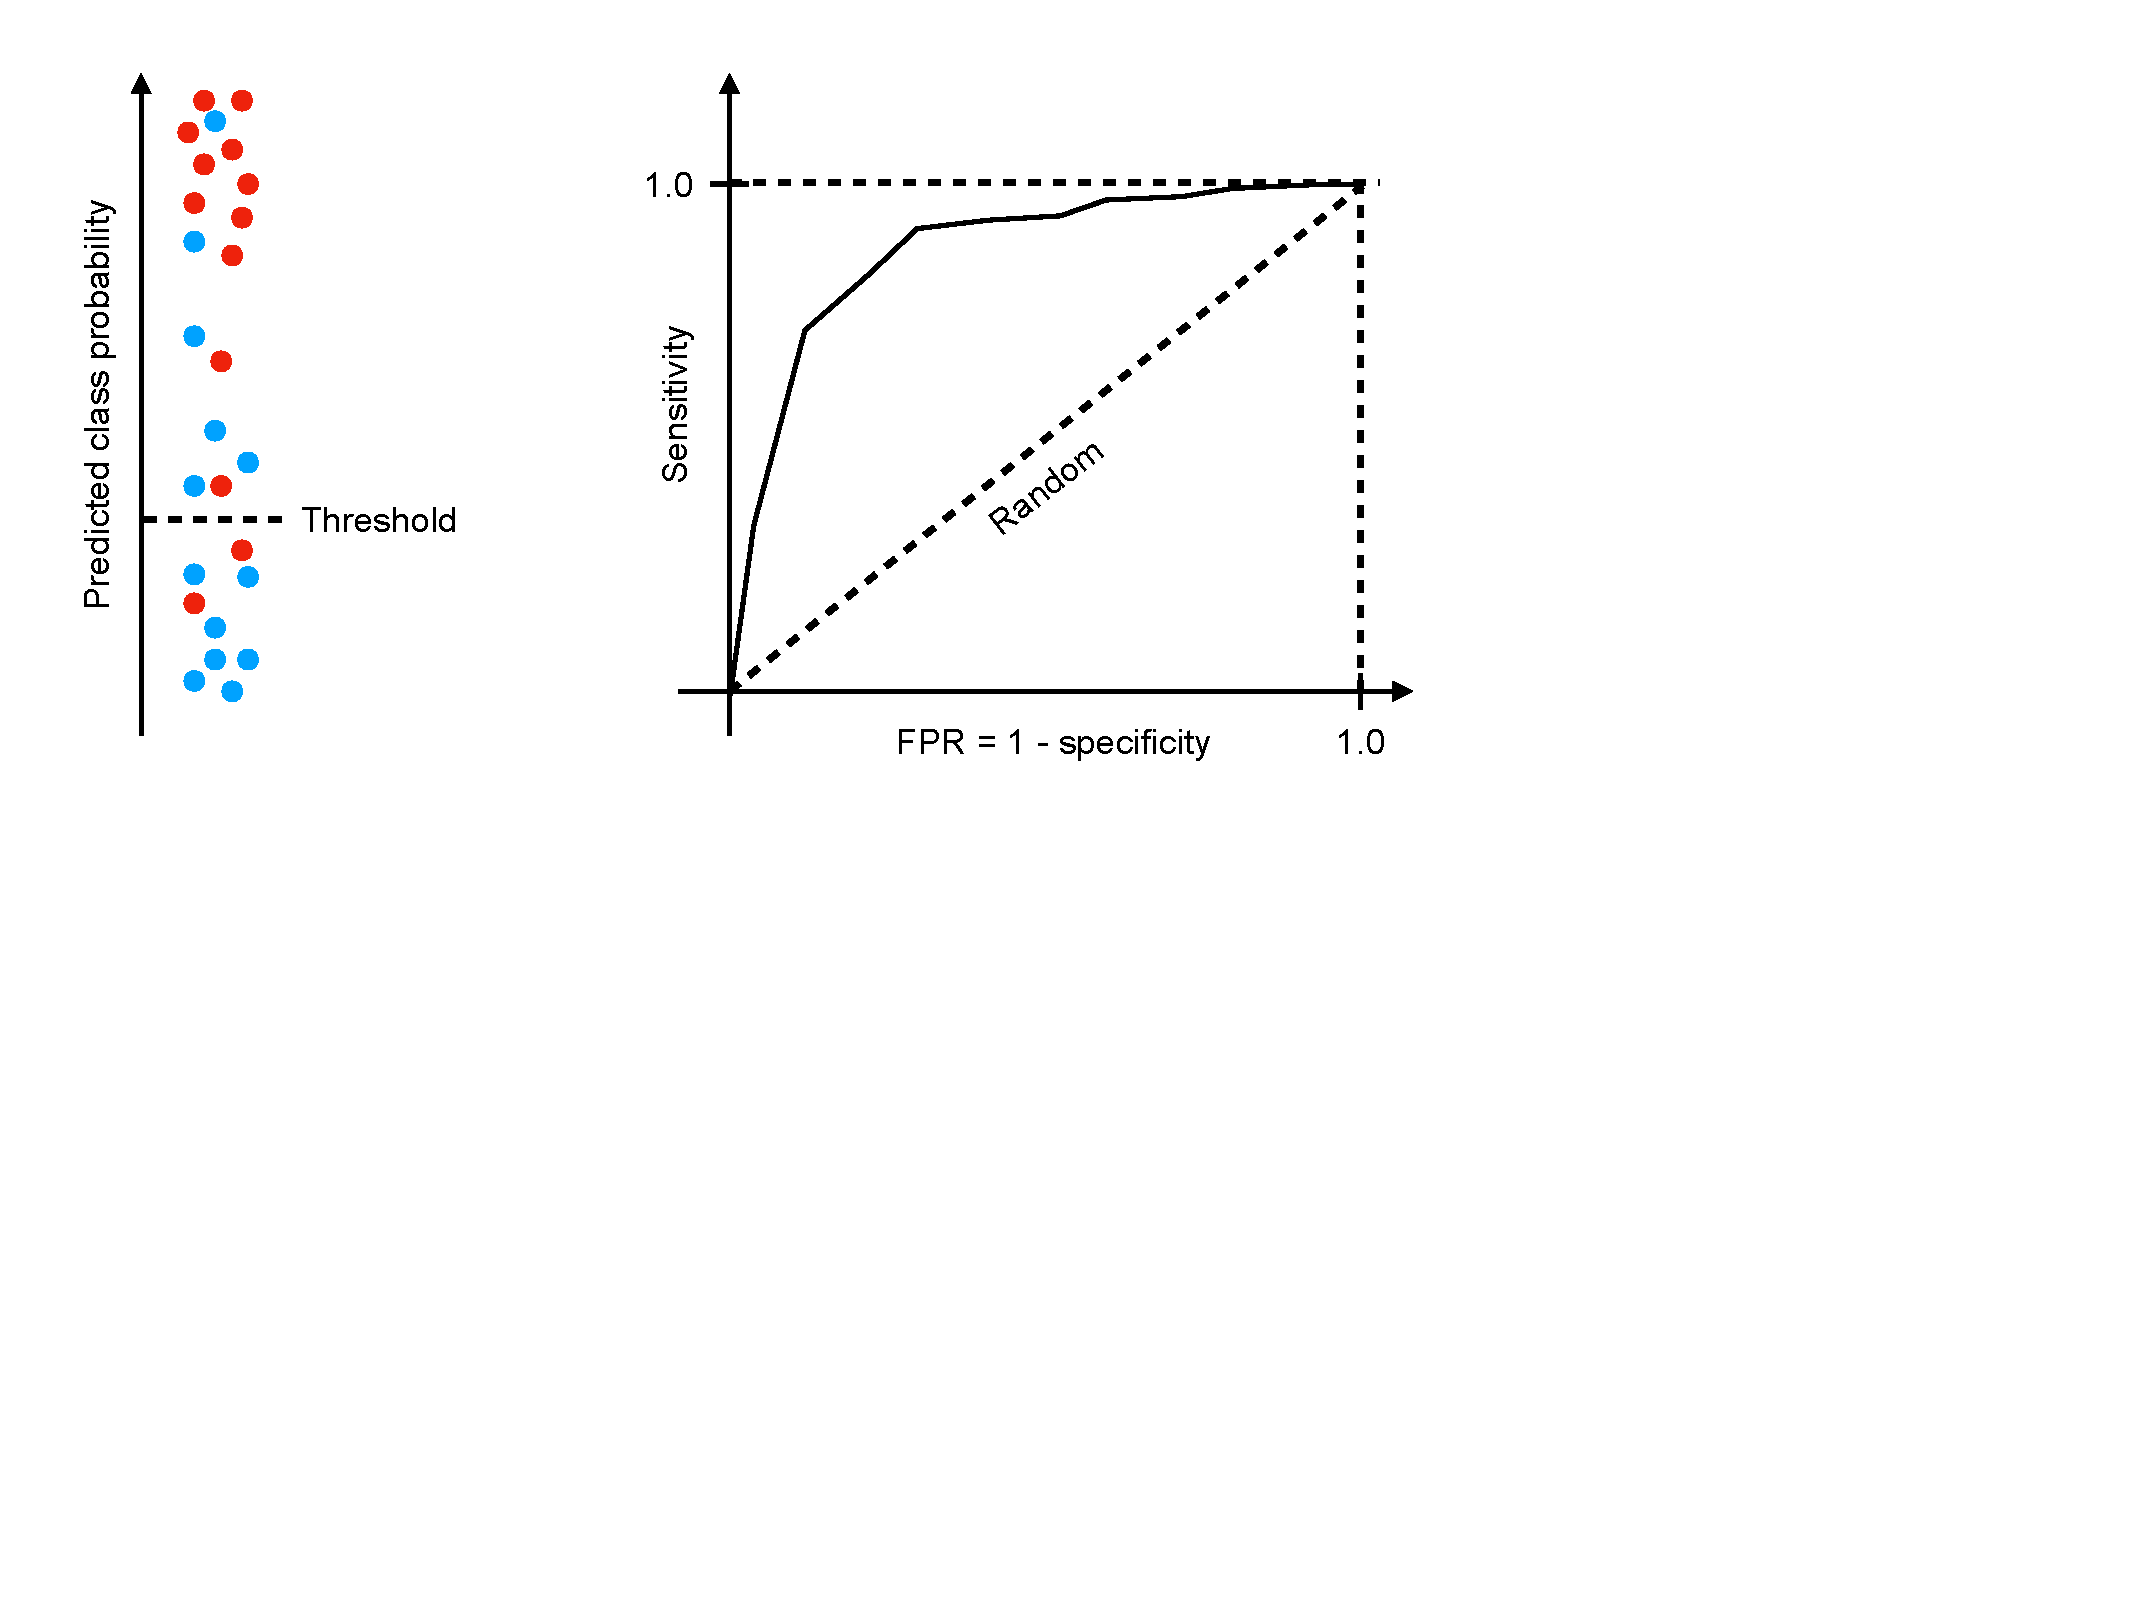
\includegraphics[width=0.6\textwidth]{../figures/ROC.pdf}
  \end{figure}
  \begin{itemize} 
    \item Une autre façon d'évaluer la performance d'un algorithme est la courbe $ROC$ (receiver operating characteristic). 
    \item Pour résumer ces courbes, on utilise l'$AUC$ (area under the curve). 
    \begin{itemize}
      \item $AUC = \frac{1}{2}$ : un classifieur aléatoire
      \item $AUC = 1$ : un classifieur parfait
    \end{itemize}
    \item L'$AUC$ est identique à l'index de concordance : la probabilité qu'une paire $(+,-)$ sera correctement ordonnée. 
  \end{itemize}
\end{frame}


\begin{frame}
  \frametitle{1.5 Évaluation d'un modèle (régression)}
  \begin{itemize}
  \item \blue{Compter} le nombre d'erreurs n'a pas de sens
    \pause
  \item Somme des carrés des erreurs : $\text{RSS} = \sum_{i=1}^n \left(y_i - f(\xvec_i) \right)^2$
  \item \tikzmark{ml0}{Racine} de l'erreur quadratique moyenne \textcolor{gray!70}{(Root Mean Squared Error)} : 
    \[\text{RMSE} = \sqrt{\frac1n \sum_{i=1}^n \left(y_i - f(\xvec_i) \right)^2}\]
  \item Erreur carrée relative : $\text{RSE} = \frac{\sum_{i=1}^n \left(y_i - f(\xvec_i) \right)^2}{\sum_{i=1}^n \left(y_i - \overline{y} \right)^2}$ \hspace{1em} $\overline{y} = \sum_{l=1}^n y_l$
  \item \tikzmark{ml1}{Coefficient} de détermination :
    \[
      R^2 = 1 - \text{RSE} = \frac{\sum_{i=1}^n \left( y_i - \overline{y} \right) \left( f(\xvec_i) - \overline{f(\xvec)} \right) }{\sqrt{\sum_{i=1}^n \left(y_i - \overline{y} \right)^2} \sqrt{\sum_{i=1}^n \left(f(\xvec_i) - \overline{f(\xvec)} \right)^2}}
    \]
  \end{itemize}
  \tikz[overlay,remember picture]{\draw[draw=MyBlue,thick]
    ($(ml0)+(-0.6,0.4)$) rectangle ($(ml0)+(11,-2.)$);}
  \tikz[overlay,remember picture]{\draw[draw=MyBlue,thick]
    ($(ml1)+(-0.6,0.4)$) rectangle ($(ml1)+(11,-2.2)$);}
\end{frame}

\begin{frame}
  \frametitle{1.6 Sélection de modèle}
  \begin{itemize}
  \item Comment déterminer \blue{le meilleur modèle} parmi ceux appris :
    \begin{itemize}
    \item avec différents algorithmes d'apprentissage ;
    \item avec différentes valeurs d'hyperparamètre(s) pour le même algorithme ?
    \end{itemize}
    \pause
  \item \black{Idée :} sélectionner celui qui a la \blue{meilleure performance sur le jeu de test.}
    \pause
  \item \black{Problème :} on ne peut plus déterminer l'\blue{erreur de
      généralisation} car les données de test ont déjà servi.
  \pause
  \item On sépare les données en 3 jeux : apprentissage, \red{validation} et test.
  \end{itemize}
  \begin{center}
    \begin{tikzpicture}
      \draw [draw=MyBlue, thick] (0.,5.5) rectangle (10.,4.5) node[pos=.5]{\blue{Jeu de données}};
      \pause
      \draw [->, draw=MyDarkGrey, line width=2] (5, 4.3) -- (5, 3.8);
      \draw [draw=MyDarkGrey, thick] (0.,3.5) rectangle (5.5,2.5) node[pos=.5]{\black{Entraînement}};
      \draw [draw=MyDarkGrey, thick] (5.5,3.5) rectangle (8.,2.5) node[pos=.5]{\black{Validation}};
      \draw [draw=MyDarkGrey, thick] (8.,3.5) rectangle (10.,2.5)  node[pos=.5]{\black{Test}};
    \end{tikzpicture}
  \end{center}
\end{frame}

\begin{frame}
  \frametitle{1.6 Sélection de modèle - jeu de validation}
  \begin{center}
    \begin{tikzpicture}
      \draw [draw=MyDarkGrey, thick] (0.,3.5) rectangle (5.5,2.5) node[pos=.5]{\black{Entraînement}};
      \draw [draw=MyDarkGrey, thick] (5.5,3.5) rectangle (8.,2.5) node[pos=.5]{\black{Validation}};
      \draw [draw=MyDarkGrey, thick] (8.,3.5) rectangle (10.,2.5)  node[pos=.5]{\black{Test}};
    \end{tikzpicture}
  \end{center}
  \begin{itemize}
  \item Le \red{jeu d'entraînement} sert à apprendre \blue{chacun des} modèles
  \item Le \red{jeu de validation} sert à \blue{sélectionner} le meilleur modèle
  \item Le \red{jeu de test} sert à estimer l'erreur de généralisation \blue{du modèle sélectionné}
  \pause
  \item \black{Problèmes :}
    \begin{itemize}
    \item On utilise seulement une fraction des données pour l'entraînement
    \item Possiblité que le modèle sélectionné ait une meilleure performance
      sur ce jeu de validation précis à cause d'un artefact.
    \end{itemize}
  \end{itemize}
\end{frame}

\begin{frame}
  \frametitle{1.6 Sélection de modèle - Validation croisée}
  \begin{itemize}
  \item On peut aussi utiliser la \blue{validation croisée} pour la \blue{sélection de modèle}
  \item On sépare le jeu d'entraînement en K \blue{blocs} (ou folds)
  \item Pour chaque algorithme ou valeur d'hyperparamètre à évaluer :
    \begin{itemize}
    \item On utilise tour à tour chacun des blocs comme \blue{jeu de
        validation} et l'union des autres comme \blue{jeu d'entraînement}
  \item[$\Rightarrow$] on obtient K scores de performance $\rightarrow$ \blue{performance moyenne} 
  \end{itemize}
\item On sélectionne l'algorithme ou la valeur d'hyperparamètre qui donne la meilleure performance moyenne
\item On réentraîne sur le jeu d'entraînement l'algorithme sélectionné
\item On estime l'erreur de généralisation en évaluant sur le jeu de test le modèle ainsi obtenu
  \end{itemize}
\end{frame}

\begin{frame}
  \frametitle{1.6 Sélection de modèle - Validation croisée}
    \begin{center}
    \small
    \begin{tikzpicture}
      \draw [draw=MyBlue, thick] (0.,7.7) rectangle (9.,7.2) node[pos=.5]{\blue{Jeu de données}};
      \pause
      \draw [->, draw=MyBlue, line width=1.5] (4.5, 7.1) -- (4.5, 6.6);
      \draw [draw=MyDarkGrey, thick] (0, 6.5) rectangle (7.5, 6)  node[pos=.5]{\black{Entraînement}};      
      \draw [draw=MyDarkGrey, thick] (7.5, 6.5) rectangle (9, 6) node[pos=.5]{\black{Test}};      
      \pause
      \draw [->, draw=MyDarkGrey, line width=1.5] (3.75, 5.9) -- (3.75, 5.4);
      \draw [draw=MyDarkGrey, thick] (0.,5.3) rectangle (1.5,4.8) node[pos=.5]{\black{Bloc 1}};
      \draw [draw=MyDarkGrey, thick] (1.5,5.3) rectangle (3.,4.8) node[pos=.5]{\black{Bloc 2}};
      \draw [draw=MyDarkGrey, thick] (3.,5.3) rectangle (4.5,4.8) node[pos=.5]{\black{Bloc 3}};
      \draw [draw=MyDarkGrey, thick] (4.5,5.3) rectangle (6.,4.8) node[pos=.5]{\black{Bloc 4}};
      \draw [draw=MyDarkGrey, thick] (6.,5.3) rectangle (7.5,4.8) node[pos=.5]{\black{Bloc 5}};
      \pause
      \draw [->, draw=MyDarkGrey, line width=1.5] (3.75, 4.7) -- (3.75, 4.2);
      \draw [draw=MyDarkGrey, thick] (0.,4.1) rectangle (1.5,3.6) node[pos=.5]{\black{Test 1}};
      \draw [draw=MyDarkGrey, thick] (1.5,4.1) rectangle (7.5,3.6) node[pos=.5]{\black{Entraînement 1}};
      \pause
      \draw [->, draw=MyOrange, thick] (7.7, 3.85) -- (8.2, 3.85) node[pos=2.1]{\red{Perf 1}};
      \pause
      \node[text width=1em] at (3.75, 3.3) {$\boldsymbol{\vdots}$};
      \draw [draw=MyDarkGrey, thick] (0.,2.8) rectangle (6,2.3) node[pos=.5]{\black{Entraînement 5}};
      \draw [draw=MyDarkGrey, thick] (6.,2.8) rectangle (7.5,2.3) node[pos=.5]{\black{Test 5}};
      \draw [->, draw=MyOrange, thick] (7.7, 2.55) -- (8.2, 2.55) node[pos=2.1]{\red{Perf 5}};
      \pause
      \draw [decorate, decoration = {brace}, draw=MyOrange, line width=2] (9.5, 3.9) --  (9.5,2.4);
      \node[text width=2em] at (10.2, 3.2) {\red{Perf moyenne}};
      \pause
      \draw [draw=MyPink, thick] (-0.1, 5.4) rectangle (11.5, 2.2) node[pos=0.32, below=60]{\color{MyPink}{Pour chaque algorithme/valeur d'hyperparamètre}};
      \pause
      \node[align=left] at (4., 1.5) {\color{MyPink}{$\rightarrow$ meilleur algorithme/valeur d'hyperparamètre}};
      \pause
      \draw [->, draw=MyPink, line width=2] (7.3, 1.7) -- (7.3, 5.9);
      \draw [draw=MyPink, line width=2, fill=MyLightGrey] (0, 6.5) rectangle (7.5, 6) node[pos=.5]{\color{MyPink}{\textbf{Ré-entraînement }}};      
      \pause
      \draw [draw=MyOrange, line width=2] (7.5, 6.5) rectangle (9, 6) node[pos=.5]{\red{Test}};      
      \draw [->, draw=MyOrange, thick] (9.1, 6.25) -- (9.6, 6.25) node[pos=3.1]{\red{Perf géné}};
    \end{tikzpicture}
  \end{center}    
\end{frame}

\begin{frame}
  \frametitle{1.6 Sélection de modèle - Validation croisée}
  \begin{itemize}
  \item Utiliser une validation croisée :
    \begin{itemize}
    \item pour \blue{la sélection de modèle} (boucle interne)
    \item et pour \blue{l'évaluation} du modèle sélectionné (boucle externe)
    \end{itemize}
  \item Peut devenir \blue{coûteux en calculs :}
    \begin{itemize}
    \item \textbf{Exemple :} si K = 5 pour la boucle interne, K=10 pour la boucle externe, et on a
      10 valeurs d'hyperparamètre à évaluer : 500 modèles à entraîner.
    \item Cependant, facile à paralléliser.
    \end{itemize}
  \end{itemize}
\end{frame}

\begin{frame}
  \frametitle{1.6 Sélection de modèle - Plusieurs hyperparamètres}
  \begin{itemize}
  \item Si plusieurs hyperparamètres sont à déterminer, on doit tester des combinaisons. 
  \item \blue{Option 1} : parcours de la grille de combinaisons (grid search)
  \item \blue{Option 2} : optimisation successive (greedy search)
  \item \blue{Option 3} : tirer aléatoirement des combinaisons (random search)
  \end{itemize}
\end{frame}


\begin{frame}
  \begin{center}
    \large{2. Régularisation}
  \end{center}
\end{frame}

\begin{frame}
  \frametitle{2.1 Régularisation}
  \begin{itemize}
  \item Par principe, la \blue{minimisation du risque empirique} conduit facilement au \blue{surapprentissage}
  \item La \red{régularisation} consiste à \blue{contraindre} le problème pour
    \blue{limiter la complexité} du modèle
    \begin{itemize}
    \item \red{Complexité} : notion théorique, par ex. Vapnik--Chervonenkis
    \item Intuitivement : « flexibilité » des modèles que l'on peut apprendre
    \item Proxys  : nombre de paramètres ; amplitude possible de ces paramètres
    \end{itemize}
    \[ \hat{f} = \argmin_{f \in \fcal} \frac1n \sum_{i=1}^n L(y_i, f(\xvec_i))
      {\color{MyOrange} \, + \, \lambda \, \Omega(f) } \hspace{1em} \lambda > 0
    \]
  \pause
  \item \red{Coefficient de régularisation} $\lambda > 0$ :
    \blue{hyperparamètre} qui gouverne l'importance relative entre la
    minimisation du risque empirique et la complexité $\Omega(f)$ du modèle.
  \end{itemize}
\end{frame}

\begin{frame}
  \frametitle{2.1 Régularisation ridge}
  \begin{itemize}
  \item Exemple 1 : \red{Régularisation ridge} (ou \red{$\ell_2$}, ou \red{weight decay})
    \begin{itemize}
    \item Pour un modèle paramètrique de paramètres $\theta_1, \theta_2, \dots, \theta_d$,
    \item[] $\Omega(\thetavec) = \ltwonorm{\thetavec} = \sum_{j=1}^d \theta_j^2$ contrôle \blue{l'amplitude des paramètres} 
      \pause
      \vspace{1em}
    \item \red{Régression ridge :}
      \[\argmin_{\betavec \in \RR^{p+1}} \frac1n 
        \left(\yvec - X \betavec \right)^\top \left(\yvec - X \betavec
        \right) + \lambda \ltwonorm{\betavec}^2 \]
    \item[] Admet toujours une unique solution
      $\betavec^* = \left(X^\top X + \lambda I_p \right)^{-1} X^\top \yvec$
      car ajouter une matrice diagonale à coefficients strictement positifs à
      $X^\top X$ la rend inversible
    \end{itemize}
  \end{itemize}
\end{frame}

\begin{frame}
  \frametitle{Chemin de régularisation}
  \begin{center}
    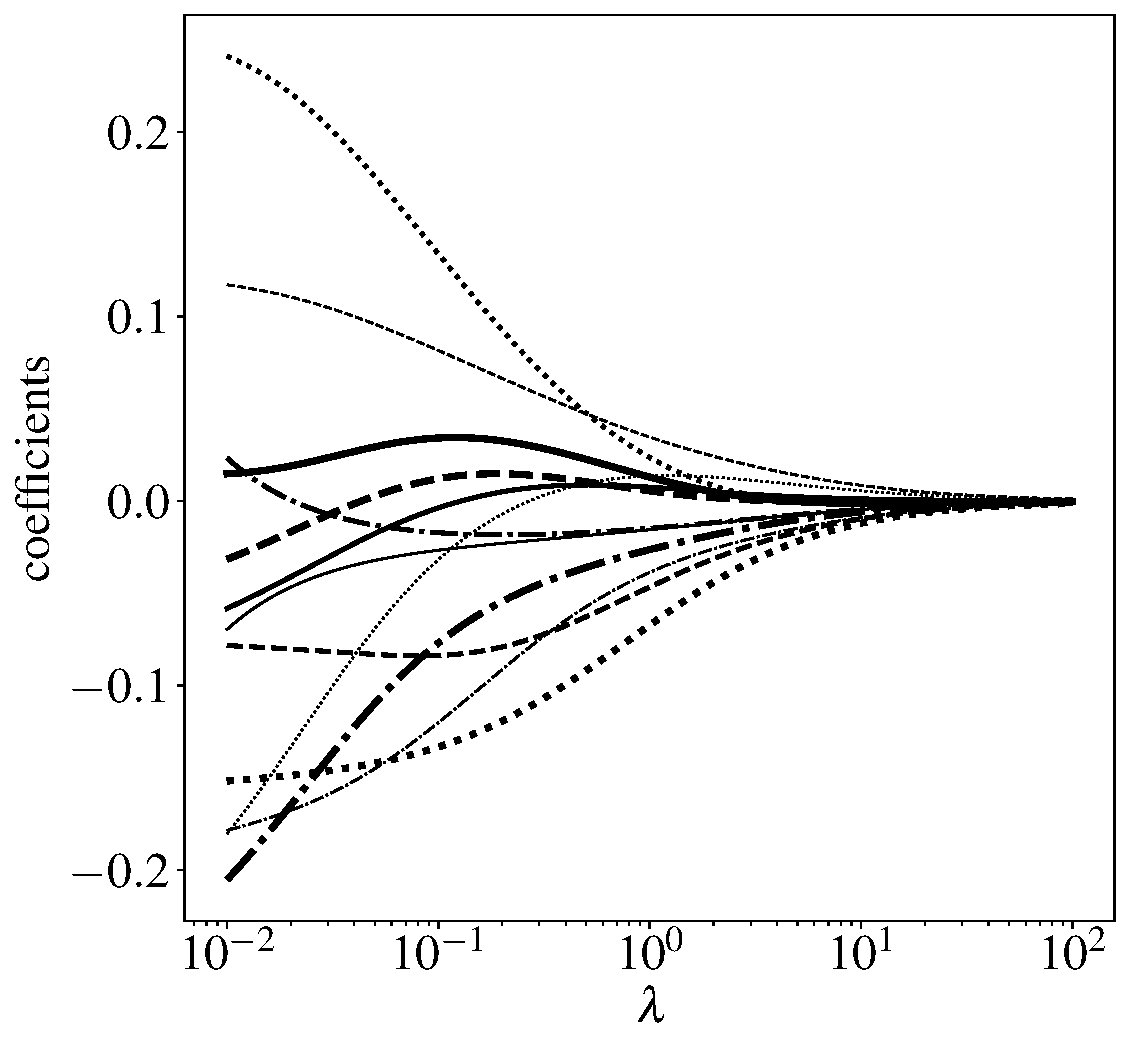
\includegraphics[width=.7\textwidth]{figures/ridge_path}  
  \end{center}
\end{frame}

\begin{frame}
  \frametitle{Interprétation géométrique}
  \begin{center}
    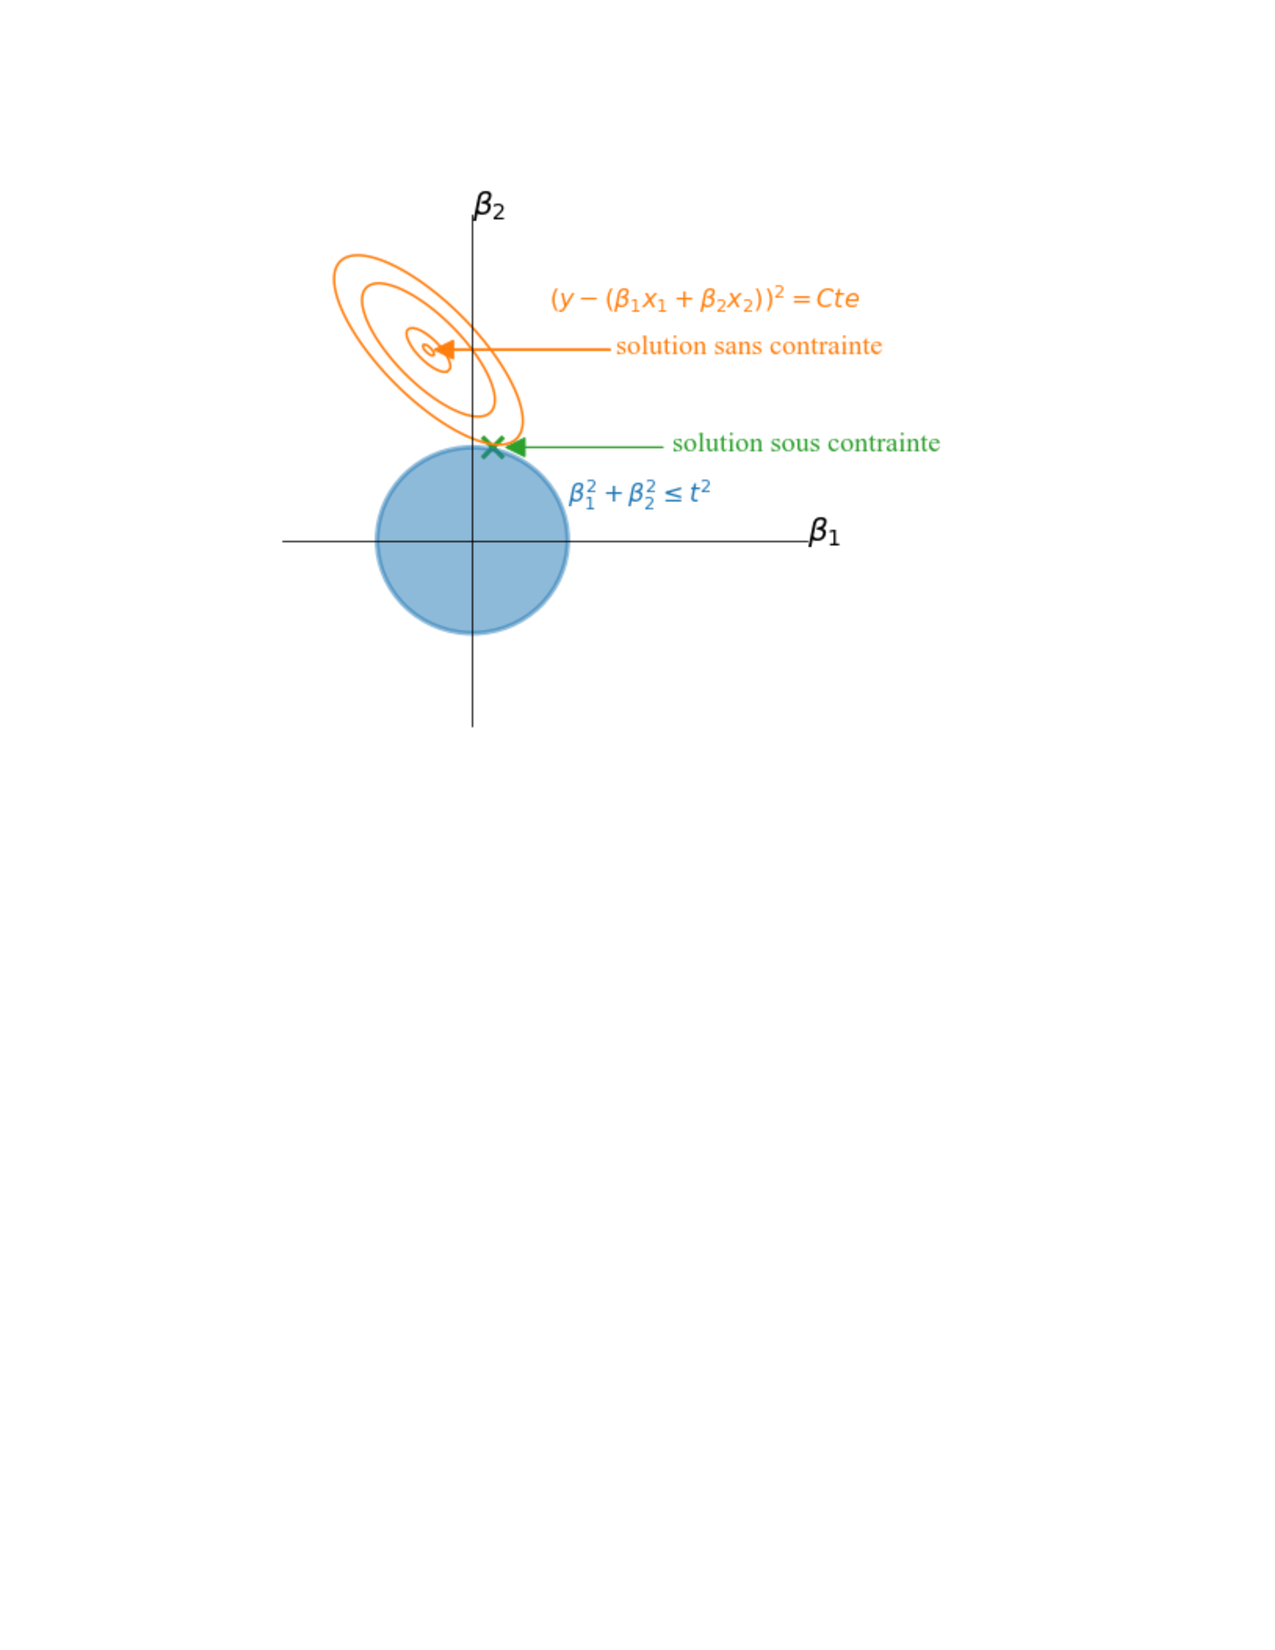
\includegraphics[width=.7\textwidth]{figures/l2reg_geom}  
  \end{center}
\end{frame}

\begin{frame}
  \frametitle{2.2 Lasso}
  \begin{itemize}
  \item Exemple 2 : \red{Régularisation $\ell_1$} 
    \begin{itemize}
    \item Pour un modèle paramètrique de paramètres $\theta_1, \theta_2, \dots, \theta_d$,
    \item[]
      $\Omega(\thetavec) = \lonenorm{\thetavec} = \sum_{j=1}^d \lvert \theta_j
      \rvert$ contrôle \blue{le nombre de paramètres non nuls} $\rightarrow$
      \red{parcimonie} \textcolor{gray!70}{(sparsity)} \pause \vspace{1em}
    \item \red{Lasso} (Least Absolute Sparse Selection Operator) :
      \[\argmin_{\betavec \in \RR^{p+1}} \frac1n 
        \left(\yvec - X \betavec \right)^\top \left(\yvec - X \betavec
        \right) + \lambda \lonenorm{\betavec} \]
    \item Résolu par l'algorithme du gradient.
    \end{itemize}
  \end{itemize}
\end{frame}

\begin{frame}
  \frametitle{Chemin de régularisation}
  \begin{center}
    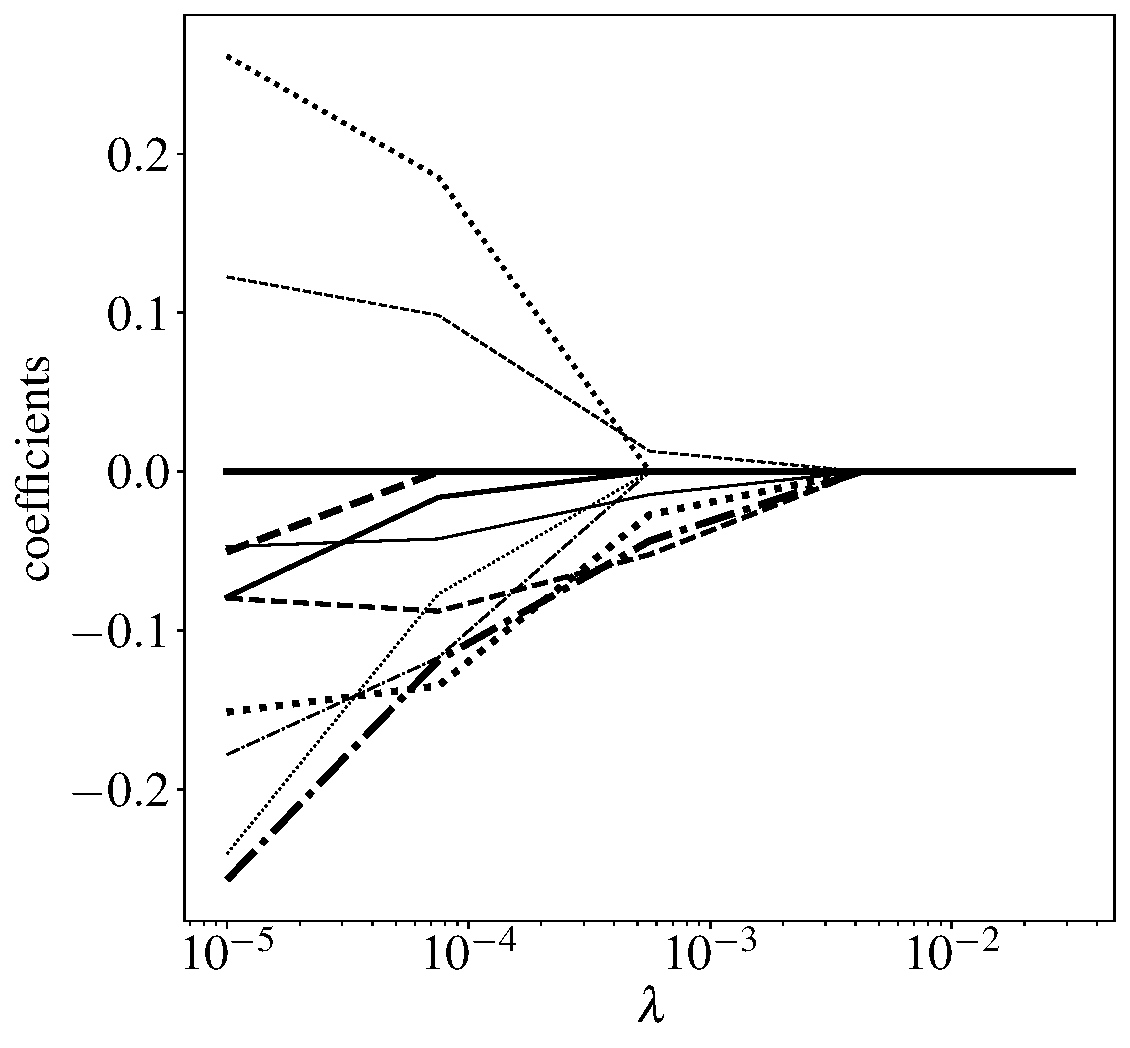
\includegraphics[width=.7\textwidth]{figures/lasso_path}  
  \end{center}
\end{frame}

\begin{frame}
  \frametitle{Interprétation géométrique}
  \begin{center}
    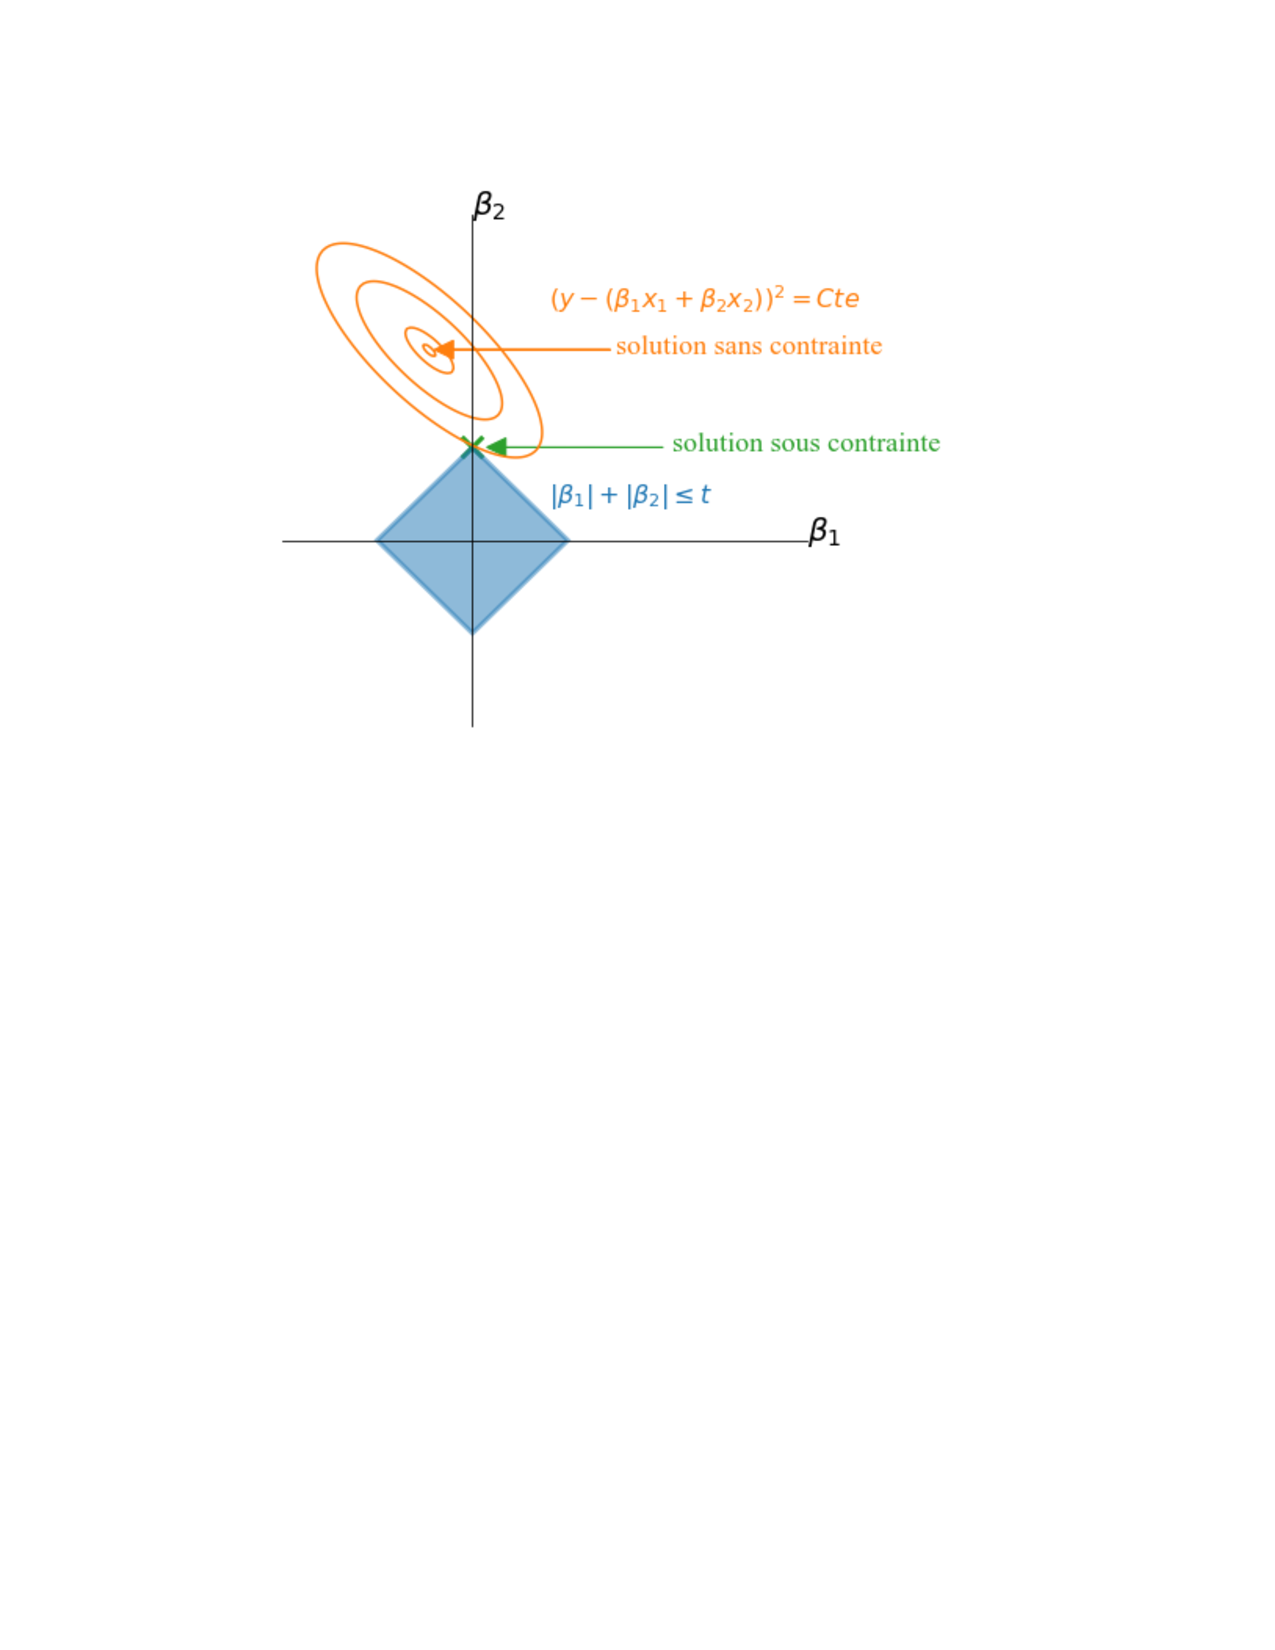
\includegraphics[width=.7\textwidth]{figures/l1reg_geom}  
  \end{center}
\end{frame}

% \begin{frame}{Exemple : ridge regression}
% \begin{figure}[htb]
% \includegraphics[width=0.6\textwidth]{../graphics/sample_from_sin.png}
% \end{figure}
% \begin{itemize}
%   \item Données : $(x_i, y_i)$ (red), we would like to build a model to predict the value $y$ for any given $x$.
%   \item The true function is $g(x)=\sin (x)$ (displayed in blue).
%   \item The measurements $y_i$ are noisy outputs of that function, i.e.
%   \begin{equation}
%   y_i = \sin (x_i) + \epsilon \; , \;\;\; \;\;\; \epsilon \sim \mathcal{N}(0,0.2)
%   \end{equation}
% \end{itemize}
% \end{frame}

% \begin{frame}{A simple example: polynomial curve fitting}
% \begin{itemize}
%   \item We use the following polynomial model:
%   \begin{eqnarray}
%   f(x) &=& a_0 + a_1 x + a_2 x^2 + \ldots + a_m x^m \nonumber \\
%   &=& \param^T \featmap (x)
%   \end{eqnarray}
%   \item Parameter vector: $\param = (a_0, a_1, \ldots, a_m)^T$
%   \item Here, the initial measurement $x$ is a scalar. In our model, we map $x$ to a higher dimensional space:
%   \begin{eqnarray}
%     \featmap : \mathbb{R}^{\nfeatures} &\rightarrow & \mathbb{R}^Q \nonumber \\
%     x &\rightarrow & \featmap (x) = (1, x, x^2, \ldots, x^m)^T
%   \end{eqnarray}
%   \item The model is linear in the parameters $\theta$ and linear in $\featmap$, but for $m>1$, the model is not linear in $x$.
% \end{itemize}
% \end{frame}

% \begin{frame}{A simple example: polynomial curve fitting}
% \begin{itemize}
%   \item One classical approach is to minimize the least squared error between measured and predicted values:
%   \begin{eqnarray}
%     \min_{\param} \loss(\param) &=& \min_{\param} \sum_{i=1}^N (y_i - f(x_i))^2 \nonumber \\
%     &=& \min_{\param} \sum_{i=1}^N (y_i - \param^T \featmap (x_i))^2
%   \end{eqnarray}
%   \item This can be achieved by setting the gradient with respect to $\param$ to zero:
%   \begin{equation}
%     \nabla_{\param} \loss = (\frac{\partial \loss}{\partial a_0}, \frac{\partial \loss}{\partial a_1}, \ldots, \frac{\partial \loss}{\partial a_m} )^T = 0
%   \end{equation}
%   \item Unlike for most optimization problems in this course, this leads to an analytical solution for $\param$. This is known as \textbf{linear regression}. For more details, we refer to \cite{Hastie2009}.
% \end{itemize}
% \end{frame}

% \begin{frame}{Overfitting and underfitting}
% \begin{columns}
% \begin{column}{.8\textwidth}
% \begin{figure}[htb]
%   \includegraphics[width=0.75\textwidth]{../graphics/polyfit_degree_1.png}
% \end{figure}
% \end{column}
% \begin{column}{.2\textwidth}
% $\| \param \|^2 = 0.67$
% \end{column}
% \end{columns}
% For $m=1$, the model is linear in its inputs. The solution is not capable of modeling the measured data points; we get a poor approximation of the original function. The family of functions we have used was not complex enough to model the true data distribution. We also speak of \textbf{underfitting}.
% %\begin{textblock}{0}(.9\textwidth,\paperheight)
% %  Test
% % \end{textblock}
% \end{frame}

% \begin{frame}{Overfitting and underfitting}
% \begin{columns}
% \begin{column}{.8\textwidth}
% \begin{figure}[htb]
%   \includegraphics[width=0.75\textwidth]{../graphics/polyfit_degree_3.png}
% \end{figure}
% \end{column}
% \begin{column}{.2\textwidth}
% $\| \param \|^2 = 1.72$
% \end{column}
% \end{columns}
% For $m=3$, we obtain a solution that seems to be quite right: it is sufficiently complex to model the true data distribution, but not too complex to model the small variations which are due to noise.
% \end{frame}

% \begin{frame}{Overfitting and underfitting}
% \begin{columns}
% \begin{column}{.8\textwidth}
% \begin{figure}[htb]
%   \includegraphics[width=0.75\textwidth]{../graphics/polyfit_degree_11.png}
% \end{figure}
% \end{column}
% \begin{column}{.2\textwidth}
% $\| \param \|^2 \approx 10^7$
% \end{column}
% \end{columns}
% For $m=11$, we obtain a solution that has zero error (the function passes through every point of the training set). But the coefficients with large absolute values that cancel each other precisely on the training points lead to a highly unstable function. We speak of \textbf{overfitting} and \textbf{poor generalization}.
% \end{frame}

% \begin{frame}{Overfitting and underfitting}
% \begin{columns}
% \begin{column}{.8\textwidth}
% \begin{figure}[htb]
%   \includegraphics[width=0.75\textwidth]{../graphics/polyfit_degree_11_N60.png}
% \end{figure}
% \end{column}
% \begin{column}{.2\textwidth}
% $\| \param \|^2 = 5647$
% \end{column}
% \end{columns}
% One way of reducing overfitting is to increase the number of samples. Even if the function is complex, it cannot be “too wild”, as it has to find a compromise between many training samples. This however implies the annotation (or measurement) of more samples.
% \end{frame}

% \begin{frame}{Overfitting and underfitting}
% \begin{columns}
% \begin{column}{.8\textwidth}
% \begin{figure}[htb]
%   \includegraphics[width=0.75\textwidth]{../graphics/ridge_regression_11_10.png}
% \end{figure}
% \end{column}
% \begin{column}{.2\textwidth}
% $\| \param \|^2 = 0.41$
% \end{column}
% \end{columns}
% Another way of preventing overfitting without increasing the number of samples, is to add a penalization term in the optimization procedure. This is also known as \textbf{regularization}:
% \begin{equation}
%   \loss = \sum_{i=1}^N (y_i - \param^T \featmap (x_i))^2 + \lambda \| \param \|^2
% \end{equation}
% \end{frame}
% % \begin{frame}
% %   \frametitle{Estimation par maximum a posteriori}
% %   \begin{center}
% %     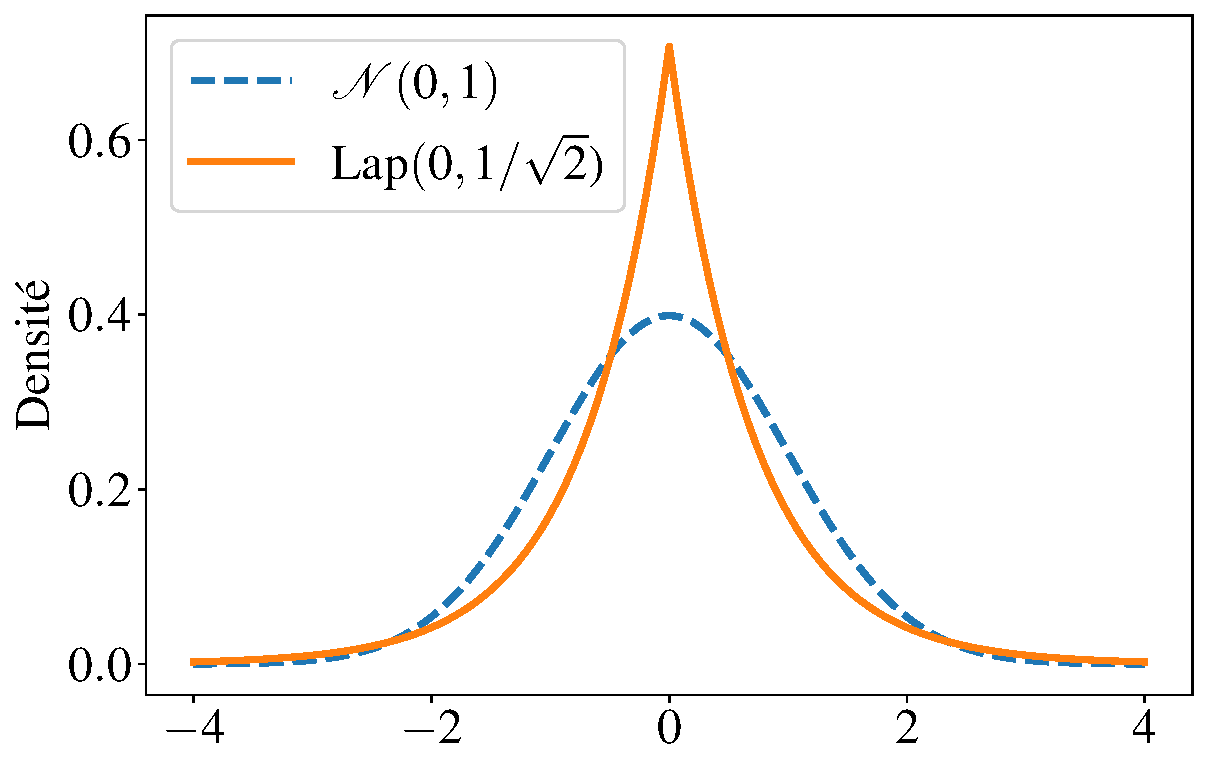
\includegraphics[width=.7\textwidth]{figures/laplace_vs_gauss}  
% %   \end{center}
% % \end{frame}

\begin{frame}
  \frametitle{Lasso: avantages}
  \begin{itemize}
  \item Réduction de dimensions d'entrée (pour $\beta_k=0$): 
  \begin{itemize}
    \item Simplification des modèles
    \item Interprétation plus simple
    \item Acquisition de moins de variables
  \end{itemize}
  \item Réduction de dimension et apprentissage au même temps. 
  \end{itemize}
\end{frame}

\begin{frame}
  \frametitle{Lasso: limitations}
  \begin{itemize}
  \item Si deux variables sont corrélées, LASSO choisira une d'entre elles. 
  \item \blue{Conséquence} : instabilité 
  \item Solution: \red{Elastic Net}
  \item[] $\Omega(\thetavec) = \alpha \ltwonorm{\thetavec} + (1-\alpha) \lonenorm{\thetavec}$
  %\item[] $\alpha \in [0, 1]$
  \end{itemize}

\end{frame}


%%% Local Variables:
%%% mode: latex
%%% TeX-master: "2022-01-azencott"
%%% End:
